\chapter{DF-054 Late-family standard Blocks}\label{record-099}

\noindent{\footnotesize\color{BookMuted}\path{docs/design/DF-054-late-family-standard-blocks.md}\par}\smallskip

\begin{RecordMeta}
title: DF-054 Late-family standard Blocks
legend: DF
lane: design
priority: medium
keywords:
  - blocks
  - component-audit
  - design-thinking
  - dogfood
  - lowerings

\end{RecordMeta}

\section{Framing}\label{record-099-framing}

The first two DOGFOOD component-family six-packs moved grouping, prose, links, dividers, text entry, choice, decision, navigation, disclosure, and path progress into typed standard Blocks. This cycle takes the remaining v7 component-family audit queue and turns it into concrete first-party Blocks with metadata, schema-bound input, command intents, ready stories, rendered output, and mode-lowering facts.

This cycle closes issues \#238 through \#243:

\begin{center}
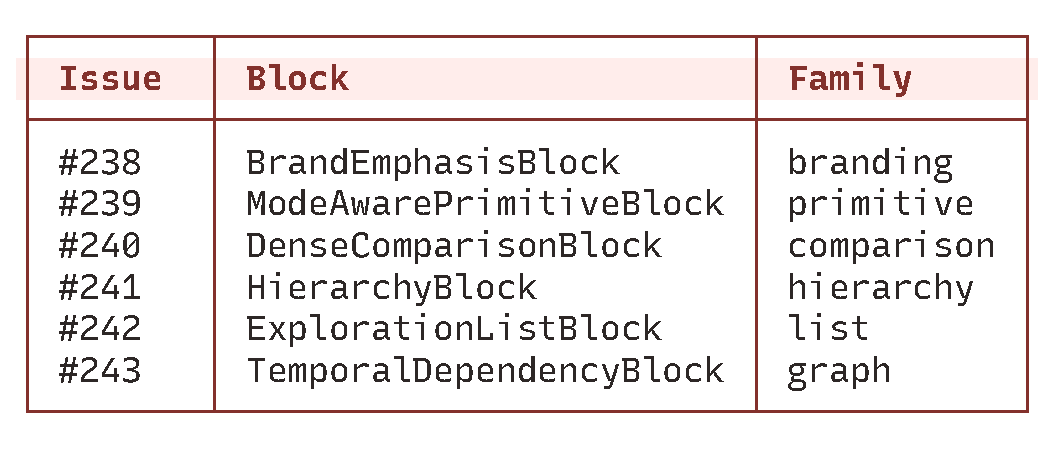
\includegraphics[width=\linewidth]{figures/tables/table-028-g1-1.pdf}
\par\smallskip{\scriptsize\color{BookMuted}Rows 1–6. Actual Bijou table component.}
\end{center}


The work follows a Design Thinking loop:

\begin{itemize}
\tightlist
\item
  observe the remaining DOGFOOD component families as reusable product semantics instead of visual one-offs
\item
  frame each family as a named Block contract with explicit data fields and facts
\item
  prototype interactive, static, pipe, and accessible shapes before treating the implementation as landed
\item
  prove catalog, schema, render, story, command, preview, and lowering behavior in tests
\end{itemize}

\section{Sponsored Users}\label{record-099-sponsored-users}

\begin{itemize}
\tightlist
\item
  TUI authors who need reusable semantics for branding, primitives, comparisons, hierarchies, exploratory lists, and dependency views.
\item
  DOGFOOD maintainers who need the Blocks preview page to show the remaining component-family families as real examples, not future-audit placeholders.
\item
  Tooling authors who inspect selected ids, semantic values, and family facts without scraping terminal layout.
\item
  Future declarative IR authors who need stable typed targets for YAML or JSON declarations.
\end{itemize}

\section{Hills}\label{record-099-hills}

\begin{enumerate}
\def\labelenumi{\arabic{enumi}.}
\tightlist
\item
  A builder can import all six Blocks and inspect metadata, data requirements, command intents, schema descriptions, and ready story ids from the public barrel.
\item
  A reader can move between visual, static, pipe, and accessible modes and recover brand, primitive, comparison, hierarchy, list, and dependency meaning without ANSI, borders, color, or animation.
\item
  A maintainer can run one DF-054 cycle test that proves the six-pack is catalogued, schema-bound, rendered, documented, and lowering-stable.
\end{enumerate}

\section{Playback Questions}\label{record-099-playback-questions}

\begin{itemize}
\tightlist
\item
  Does each late-family audit now have a named Block contract instead of a broad review note?
\item
  Are required fields concrete enough for DOGFOOD previews and small enough for reuse?
\item
  Do lower modes expose stable facts for block identity, family, variant, mode, selected value, and semantic values?
\item
  Does the DOGFOOD Blocks page have sample slots for every new definition?
\item
  Does this keep future YAML/JSON IR as an adapter over typed Block APIs?
\end{itemize}

\section{Block Contracts}\label{record-099-block-contracts}

\begin{center}
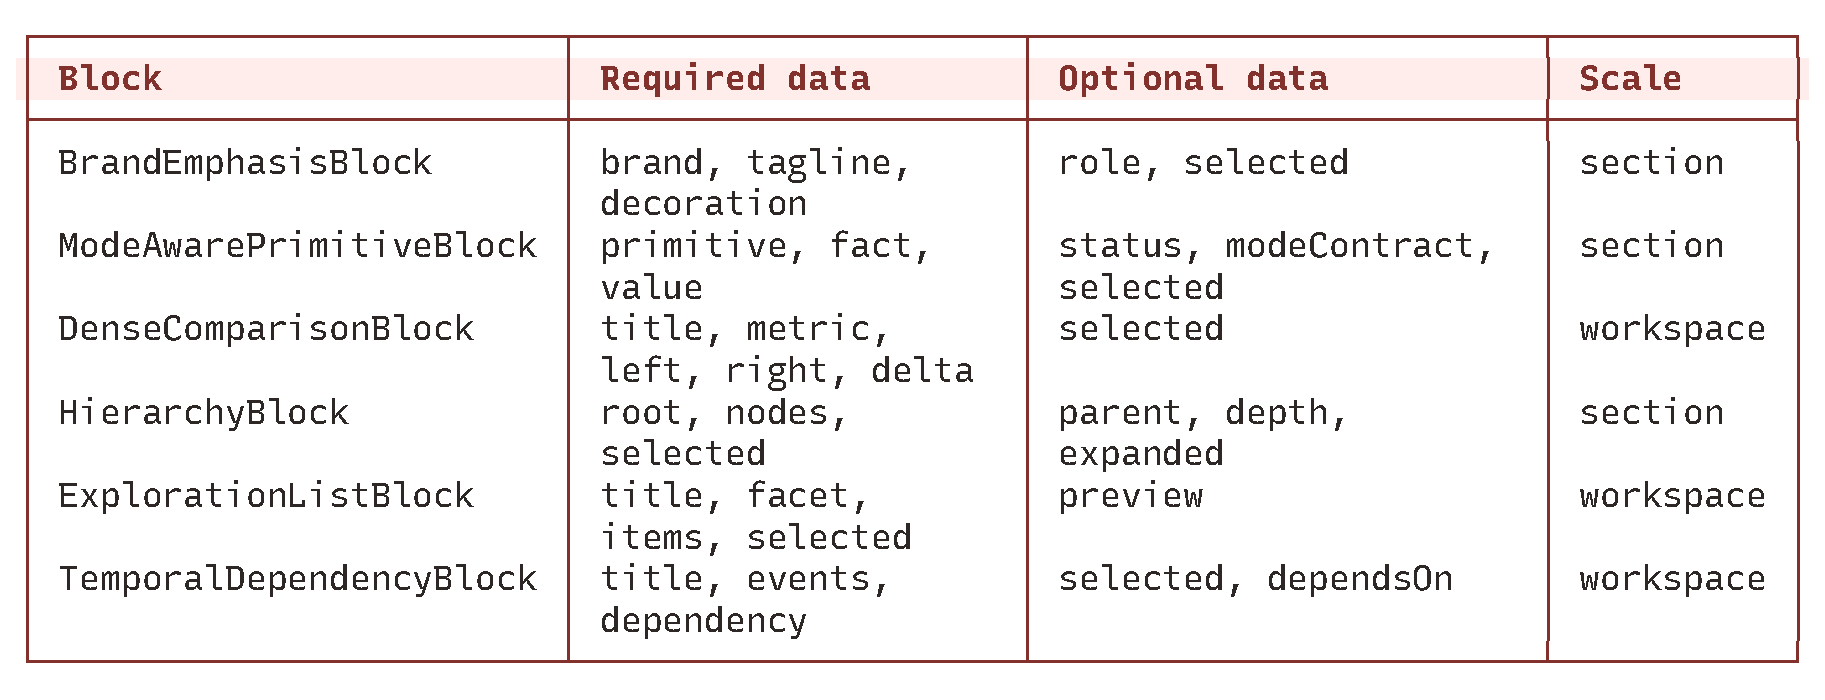
\includegraphics[width=\linewidth]{figures/tables/table-029-g1-1.pdf}
\par\smallskip{\scriptsize\color{BookMuted}Rows 1–6. Actual Bijou table component.}
\end{center}


Each Block gets the same first-party command contract:

\begin{CodeBlock}
<blockPrefix>.select
<blockPrefix>.copyFacts
<blockPrefix>.openStory
\end{CodeBlock}

\section{TUI Mockups}\label{record-099-tui-mockups}

Brand emphasis:

\begin{CodeBlock}
+-- BrandEmphasisBlock -----------------------------+
| Brand                                              |
|   BIJOU                                            |
| Tagline                                            |
|   Terminal-native app blocks                       |
| Decoration                                         |
|   accent rule                                      |
| Role                                               |
|   nonessential                                     |
+----------------------------------------------------+
\end{CodeBlock}

Mode-aware primitive:

\begin{CodeBlock}
+-- ModeAwarePrimitiveBlock ------------------------+
| Primitive                                          |
|   metric badge                                     |
| Fact                                               |
|   latency-ms                                       |
| Value                                              |
|   42                                               |
| Status                                             |
|   good                                             |
| Mode contract                                      |
|   visual and pipe                                  |
+----------------------------------------------------+
\end{CodeBlock}

Dense comparison:

\begin{CodeBlock}
+-- DenseComparisonBlock ---------------------------+
| Title                                              |
|   Compare packages                                 |
| Metric                                             |
|   tests                                            |
| Left                                               |
|   1820                                             |
| Right                                              |
|   640                                              |
| Delta                                              |
|   +12                                              |
+----------------------------------------------------+
\end{CodeBlock}

Hierarchy:

\begin{CodeBlock}
+-- HierarchyBlock ---------------------------------+
| Root                                               |
|   docs/                                            |
| Nodes                                              |
|   design/; DX-031.md; METHOD.md                    |
| Selected                                           |
|   design/                                          |
| Parent                                             |
|   docs/                                            |
| Depth                                              |
|   1                                                |
+----------------------------------------------------+
\end{CodeBlock}

Exploration list:

\begin{CodeBlock}
+-- ExplorationListBlock ---------------------------+
| Title                                              |
|   Explore components                               |
| Facet                                              |
|   input                                            |
| Items                                              |
|   TextEntry field input; SingleChoice radio/select |
| Selected                                           |
|   TextEntry                                        |
| Preview                                            |
|   field input                                      |
+----------------------------------------------------+
\end{CodeBlock}

Temporal dependency:

\begin{CodeBlock}
+-- TemporalDependencyBlock ------------------------+
| Title                                              |
|   Timeline                                         |
| Events                                             |
|   09:00 build; 09:05 test; 09:10 publish           |
| Dependency                                         |
|   publish waits for test                           |
| Selected                                           |
|   publish                                          |
| Depends on                                         |
|   test                                             |
+----------------------------------------------------+
\end{CodeBlock}

\section{Lower Modes}\label{record-099-lower-modes}

Static mode keeps the same surface structure as interactive mode and stays render-only.

Pipe mode lowers every Block to a compact record:

\begin{CodeBlock}
BrandEmphasisBlock
brand: BIJOU
tagline: Terminal-native app blocks
decoration: accent rule
role: nonessential
selected: BIJOU
\end{CodeBlock}

\begin{CodeBlock}
TemporalDependencyBlock
title: Timeline
events: 09:00 build; 09:05 test; 09:10 publish
dependency: publish waits for test
selected: publish
dependsOn: test
\end{CodeBlock}

Accessible mode lowers every Block to label-first prose:

\begin{CodeBlock}
BrandEmphasisBlock
Brand: BIJOU
Tagline: Terminal-native app blocks
Decoration: accent rule
Role: nonessential
Selected: BIJOU
\end{CodeBlock}

\begin{CodeBlock}
TemporalDependencyBlock
Title: Timeline
Events: 09:00 build; 09:05 test; 09:10 publish
Dependency: publish waits for test
Selected: publish
Depends on: test
\end{CodeBlock}

Every lower mode carries inspectable facts:

\begin{CodeBlock}
block = BrandEmphasisBlock
block.rendered = true
block.family = branding
block.variant = ready
block.mode = pipe
block.selected = BIJOU
semanticValue.brand = BIJOU
\end{CodeBlock}

\begin{CodeBlock}
block = TemporalDependencyBlock
block.rendered = true
block.family = graph
block.variant = ready
block.mode = accessible
block.selected = publish
semanticValue.title = Timeline
\end{CodeBlock}

\section{Accessibility And Directionality}\label{record-099-accessibility-and-directionality}

The first slice does not add bespoke focus behavior. The Blocks expose labels, selected values, and section values so accessible output preserves meaning when visual emphasis, indentation, dense columns, list focus, and graph arrows are removed. Text is stored as plain strings or string arrays, leaving locale, bidirectional rendering, and translation concerns to callers and localization adapters.

\section{Agent Inspectability}\label{record-099-agent-inspectability}

Agents and tests should inspect metadata, data contracts, schema descriptions, command intent ids, ready story ids, and lowering facts. They should not infer hierarchy depth from indentation, compare values from column positions, or dependency meaning from arrows.

\section{Declarative IR Note}\label{record-099-declarative-ir-note}

The Bijou IR idea remains an adapter layer over this typed API. This cycle does not introduce a new YAML or JSON runtime, but it gives future IR work concrete targets:

\begin{CodeBlock}
block: TemporalDependencyBlock
package: "@flyingrobots/bijou"
story: temporal-dependency.ready
data:
  title: Timeline
  events:
    - 09:00 build
    - 09:05 test
    - 09:10 publish
  dependency: publish waits for test
  selected: publish
  dependsOn: test
commands:
  - temporalDependency.select
  - temporalDependency.copyFacts
  - temporalDependency.openStory
facts:
  block.family: graph
  block.variant: ready
  block.selected: publish
  semanticValue.title: Timeline
\end{CodeBlock}

\section{Tests}\label{record-099-tests}

\begin{itemize}
\tightlist
\item
  \texttt{t\allowbreak{}e\allowbreak{}s\allowbreak{}t\allowbreak{}s\allowbreak{}/\allowbreak{}c\allowbreak{}y\allowbreak{}c\allowbreak{}l\allowbreak{}e\allowbreak{}s\allowbreak{}/\allowbreak{}D\allowbreak{}F\allowbreak{}-\allowbreak{}0\allowbreak{}5\allowbreak{}4\allowbreak{}/\allowbreak{}d\allowbreak{}o\allowbreak{}g\allowbreak{}f\allowbreak{}o\allowbreak{}o\allowbreak{}d\allowbreak{}-\allowbreak{}l\allowbreak{}a\allowbreak{}t\allowbreak{}e\allowbreak{}-\allowbreak{}f\allowbreak{}a\allowbreak{}m\allowbreak{}i\allowbreak{}l\allowbreak{}y\allowbreak{}-\allowbreak{}s\allowbreak{}i\allowbreak{}x\allowbreak{}-\allowbreak{}p\allowbreak{}a\allowbreak{}c\allowbreak{}k\allowbreak{}.\allowbreak{}t\allowbreak{}e\allowbreak{}s\allowbreak{}t\allowbreak{}.\allowbreak{}t\allowbreak{}s} proves all six Blocks publish through the standard catalog and package manifest.
\item
  The cycle test validates metadata, command intent shape, schema binding, accessor rejection, visual rendering, lower-mode rendering, semantic facts, and Method documentation.
\item
  DX-031 catalog tests prove the public barrel, first-party manifest, story ids, and rendered lowering checks include the expanded standard block set.
\item
  DOGFOOD Blocks page tests prove the preview navigation and per-block preview output derive from \texttt{s\allowbreak{}t\allowbreak{}a\allowbreak{}n\allowbreak{}d\allowbreak{}a\allowbreak{}r\allowbreak{}d\allowbreak{}B\allowbreak{}l\allowbreak{}o\allowbreak{}c\allowbreak{}k\allowbreak{}s}.
\end{itemize}

\section{Closeout}\label{record-099-closeout}

The six-pack is landed when:

\begin{itemize}
\tightlist
\item
  \texttt{@\allowbreak{}f\allowbreak{}l\allowbreak{}y\allowbreak{}i\allowbreak{}n\allowbreak{}g\allowbreak{}r\allowbreak{}o\allowbreak{}b\allowbreak{}o\allowbreak{}t\allowbreak{}s\allowbreak{}/\allowbreak{}b\allowbreak{}i\allowbreak{}j\allowbreak{}o\allowbreak{}u} exports all six Block definitions, schema adapters, and schema-bound block definitions
\item
  DOGFOOD Blocks preview has concrete sample slots for all six names
\item
  \texttt{s\allowbreak{}t\allowbreak{}a\allowbreak{}n\allowbreak{}d\allowbreak{}a\allowbreak{}r\allowbreak{}d\allowbreak{}B\allowbreak{}l\allowbreak{}o\allowbreak{}c\allowbreak{}k\allowbreak{}s}, \texttt{s\allowbreak{}t\allowbreak{}a\allowbreak{}n\allowbreak{}d\allowbreak{}a\allowbreak{}r\allowbreak{}d\allowbreak{}B\allowbreak{}l\allowbreak{}o\allowbreak{}c\allowbreak{}k\allowbreak{}S\allowbreak{}t\allowbreak{}o\allowbreak{}r\allowbreak{}i\allowbreak{}e\allowbreak{}s}, and \texttt{s\allowbreak{}t\allowbreak{}a\allowbreak{}n\allowbreak{}d\allowbreak{}a\allowbreak{}r\allowbreak{}d\allowbreak{}B\allowbreak{}l\allowbreak{}o\allowbreak{}c\allowbreak{}k\allowbreak{}P\allowbreak{}a\allowbreak{}c\allowbreak{}k\allowbreak{}a\allowbreak{}g\allowbreak{}e\allowbreak{}M\allowbreak{}a\allowbreak{}n\allowbreak{}i\allowbreak{}f\allowbreak{}e\allowbreak{}s\allowbreak{}t} include the six names
\item
  CHANGELOG, BEARING, and ROADMAP record the v7 late-family slice
\item
  PR text closes \#238, \#239, \#240, \#241, \#242, and \#243
\end{itemize}

